\documentclass[10pt,twocolumn]{witseiepaper}

% All KJN's macros and goodies (some shameless borrowing from SPL)

\usepackage{KJN}
\usepackage{amsmath,amsfonts}
\usepackage{listings} 
\usepackage{tikz}
\usepackage{verbatim}
\usetikzlibrary{shapes.arrows}
\usetikzlibrary{shapes.geometric}
\usetikzlibrary{plotmarks}
\usetikzlibrary{matrix}
\usepackage{pgfplots}
\usepackage{circuitikz}
\usepackage{pdfpages}
\usepackage{placeins}
\usepackage{dblfloatfix}
\usepackage{graphicx}
\usepackage{caption}
\usepackage{subcaption}
\usepackage{url}
\usepackage{cleveref}
\usepackage{color,soul}

\pagestyle{plain}

\addtolength{\oddsidemargin}{-.3in}
\addtolength{\evensidemargin}{-.3in}
\addtolength{\textwidth}{0.75in}

\addtolength{\topmargin}{-.3in}
\addtolength{\textheight}{0.1in}

%%%%%%%%%%%%%%%%%%%%%%%%%%%%%%%%%%%%%%%%%%%%%%%%%%%
\begin{document}
	
	
\title{ELEN4006 - Measurement Systems \\ The Design of a Potentiometric Smart Transducer
	for Electric Vehicle Roll Angle Estimation}
	
\author{Jared Ping (704447) \& Matthew van Rooyen (706692)
	\thanks{School of Electrical \& Information Engineering, University of the
			Witwatersrand, Private Bag 3, 2050, Johannesburg, South Africa}
}
	
	
%%%%%%%%%%%%%%%%%%%%%%%%%%%%%%%%%%%%%%%%%%%%%%%%%%%
\abstract{}
	
\keywords{Roll Angle, Potentiometer, Anti-aliasing Filter, Wheatstone Bridge, Analog-to-Digital Conversion}
	
	
\maketitle
	
%%%%%%%%%%%%%%%%%%%%%%%%%%%%%%%%%%%%%%%%%%%%%%%%%%%%
	
\section{INTRODUCTION}

Over the last decade, the ever-increasing detrimental effects of $\text{CO}_2$ emissions on the environment has become a much greater problem. This has facilitated massive growth in the electrification of transportation mediums and, in particular, electric vehicles. This new technology has provided substantial improvements in vehicle and driver active safety control systems.

Vehicle active safety control systems have become increasingly important as a method of reducing the number of motor vehicle accidents on the roads. One such measure is the roll stability control system which automatically responds when a high roll-over risk is detected. This is achieved by controlling the torque applied to the wheels of the vehicle to prevent any uncontrolled handling conditions. The system works by analysing the angle differential between the wheel base and the road surface. This angle can then be used in order to ascertain when intervention is needed by the control system.

The objective of this project is to investigate the design a potentiometric smart transducer in order to calculate the roll angle of a vehicle and the effects that the given system will have on the active safety control system. Sensors comprised of potentiometers are often used in accurately measuring angular displacement\cite{Bentley}. A potentiometer consists of a device placed within resistive coating which makes use of variable resistance to provide a measurable change in potential across the resistive element. The device can be calibrated according to the resistance per unit length which remains constant. The resistance is directly proportional to this length and thus enables the transducer to convert displacement into resistance.

The proposed solution utilities a high-bandwidth measurement system in order to accurately measure fast changing parameters of the system. These include instantaneous torque changes, volatile turbulence, and sudden impact. Thus, the measurement system will require a much larger bandwidth than the minimum $100~\mathrm{Hz}$ specified for the design to accurately poll the required system components.

This report documents the design and analysis of the proposed measurement system. The static and dynamic system characteristics will be described along with costing and error analysis. Finally, future improvements will also be considered.

\section{PROJECT DETAILS}

\subsection{Success Criteria}

The success criteria of the measurement system will be determined by the level of fulfillment of the following specifications:

\begin{itemize}
	\item A complete, critically-analyzed design of a smart transducer measurement system has been exhibited which meets a satisfactory engineering level.
	\item The system contains all elements set out by Bentley's generalized model of a measurement system.
	\item The error analysis of the system complies with industry standards.
	\item The design is both energy and cost efficient.
	\item The system bandwidth exceeds a minimum of $100~\mathrm{Hz}$.
\end{itemize}

\subsection{Assumptions}

The following assumptions were made when designing the measurement system:

\begin{itemize}
	\item It is assumed that there is no limitation on the total cost of the measurement element.
	\item The operating temperature range is expected to be within typical regions for an electric vehicle.
	\item Chosen system components can be obtained locally.
\end{itemize}

\subsection{Constraints}

The following constraints were taken into account when designing the measurement system:
\begin{itemize}
	\item The system should be designed with a bandwidth of at least $\mathrm{100~Hz}$.
	\item The system should not exhibit an overall error of more than 10~\%.
	\item The proposed installation of the system should comply with vehicle modification and safety regulations.
\end{itemize}

\section{SYSTEM DESIGN}

\subsection{Overview}

The system was designed according to Bentley's general structure of a measurement system. \figref{fig:block} shows a block diagram of the system, showing the sensing, signal conditioning, signal processing, and data presentation elements.

\begin{figure*}[]
	\centering
	\includegraphics[width=\textwidth]{Block.png}
	\vspace{0.15cm}
	\caption{System block diagram, showing the elements of Bentley's general structure of a measurement system.}
	\label{fig:block}
\end{figure*}

The system takes an input in the form of angular displacement. Using a potentiometer, this is then converted into a relative resistance. A Wheatstone bridge makes the conversion from resistance to voltage which is measured by an instrumentation amplifier. This signal is then filtered to reduce the aliasing error before being sampled by an ADC for processing with a PIC micro-controller. The microprocessor then produces an output which is read into the active safety control system after which a decision can be made by the system. \figref{fig:flow} indicates the flow diagram representing the interaction between elements.

\begin{figure}[h!]
	
	\centering
	\tikzstyle{dec} = [diamond, color=black, draw,
	text width=3em, text badly centered, node distance=2cm, inner sep=0pt]
	\tikzstyle{block} = [rectangle, draw,
	text width=12em, text centered, color=black, minimum height=2em]
	\tikzstyle{line} = [draw, very thick, color=black, ->]
	\tikzstyle{begin} = [circle, color=black, draw, node distance=1cm,
	minimum height=2em, fill=black]        
	\tikzstyle{end} = [circle ,draw, fill=black, node distance=1cm, minimum height=1.5em]
	
	\begin{tikzpicture}[scale=0.65, transform shape, node distance = 0cm, auto,>=triangle 45] 
	\draw
	node at (0,1) [begin] (begin) {}
	node at (0, -1) [dec] (gamerun) {}
	node at (1.5,-1.75) [] (pt2) {[\textsc{Engine On}]}
	node at (-2,-0.75) [] (pt3) {[\textsc{Engine Off}]}
	node at (0, -2.5) [block] (sens1) {\textsc{Potentiometer 1 Input}}
	node at (0, -4) [block] (sens2) {\textsc{Potentiometer 2 Input}}
	node at (0, -5.75) [block] (comp) {\textsc{Measurements \\ Comparison}}
	node at (0, -7.5) [dec] (withinTol) {}
	node at (2.1,-8) [] (pt4) {[\textsc{!withinTolerance}]}
	node at (2.3,-7.25) [] (pt5) {[\textsc{withinTolerance}]}
	node at (0,-9.2) [block] (prev) {\textsc{Compare to previous measurements}}
	node at (0,-11) [dec] (sensErr) {}
	node at (2.3,-10.75) [] (pt4) {[\textsc{!sensorError}]}
	node at (1.8,-11.5) [] (pt5) {[\textsc{sensorError}]}
	node at (0,-12.6) [block] (alert) {\textsc{System Intervention Required}}
	node at (5, -7.5) [begin, fill=white] (join) {}
	node at (5,-5.75) [block] (close) {\textsc{Write to memory}}
	node at (5, -2.5) [block] (disp) {\textsc{Input to Computer}}
	node at (5, -11.0) [begin, fill=white] (join2) {}
	node at (-4, -1) [end] (end1) {}
	node at (-4,-1) [begin, fill=none] (end2) {}
	node at (-4, -2.5) [coordinate] (pt) {}
	; 
	
	\draw[->] (begin) -- (gamerun);
	\draw[->] (gamerun) -- (sens1);
	\draw[->] (sens1) -- (sens2);
	\draw[->] (sens2) -- (comp);
	\draw[->] (comp) -- (withinTol);
	\draw[->] (withinTol) -- (prev);
	\draw[->] (prev) -- (sensErr);
	\draw[->] (sensErr) -- (join2);
	\draw[->] (withinTol) -- (join);
	\draw[->] (join) -- (close);
	\draw[->] (close) -- (disp);
	\draw[->] (disp) |- (gamerun);
	\draw[->] (gamerun) -- (end2);
	\draw[->] (sensErr) -- (alert);
	\draw[->] (alert) -| (join2);
	\draw[->] (join2) -- (join);
	
	\end{tikzpicture}
	\vspace{0.5cm}
	\caption{Main measurement processing algorithm}
	\label{fig:flow}
\end{figure}

Circuit diagrams for both the Wheatstone bridge and anti-aliasing filter can be found in \textit{Appendix A}. Furthermore, the circuit diagram for the overall measurement design can be found in \textit{Appendix A}.

\subsection{Sensor}

The sensor is responsible for taking the angular displacement and converting it into an electrical signal which can be outputted to the rest of the system. The rotary potentiometer, as shown in \cref{fig:pot}, contains four primary components: the resistive track, the contact/wiper, the actuator/shaft and the terminations.

\begin{figure}[h!]
	\centering
	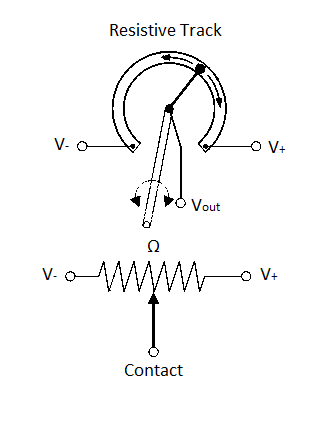
\includegraphics[width=0.35\textwidth]{Pot2.png}
	\caption{Physical design of a rotary potentiometer}
	\label{fig:pot}
\end{figure}

The sensor is connected to the wheel base of the car via the actuator. The actuator is a steel shaft with density $\mathrm{\rho_{st}} =  7~850~\mathrm{kg/m^3}$, shear modulus $\mathrm{G_{st}} = 79.3~\mathrm{GPa}$, and radius $2.6~\mathrm{mm} $. This shaft is connected directly to the contact which moves along the resistive material providing the drive interface for the sensor. As the angle of elevation of the wheel base varies, a resultant resistance is produced according to the position of the contact along the resistive track. The contact will use a copper multiple-fingered equidistant wiper along the material. This will minimize current crowding along the resistive material reducing the amount of distortion incurred\cite{handbook}.

The resistive track is made up of a conductive plastic material with a carbon black inert filler. The conductive plastic provides a much more accurate linearity in comparison to other resistive elements such as wire wound or cermet potentiometers due to its manufacturing process. It also provides a low contact resistance variation and smoother surface for the contact to move across \cite{handbook}. The total length of the resistance band must account for the total range of angular displacement allowed for by the control system. The angular displacement range in which non-critical roll-over risk occurs is between $-15 \degree \mathrm{~to~} 15 \degree $. This translates to a potentiometer resistance range of $ 30 \degree$ with a buffer of $1 \degree $ to allow for any error or over-extension of the wheel base. 

The terminations will be connected to the rest of the circuit using a solder connection. This provides the advantage of increased reliability and reduces the amount of inductance incurred at the terminations. Furthermore, the solder method provides redundant connection to the resistive track, increasing it's ability to handle severe vibrations and thus increasing its durability\cite{TIinstr}.
 
\subsubsection{Mechanical Model}

A mass-spring-damper model of the potentiometer has been used to determine a ratio between the torque and the roll angle output. The conversion between the two states is modelled using a second-order transfer function that considers the friction, spring, damping and inertia experienced by the steel shaft, as shown in \eqnref{mech_model}.
\begin{equation}
\mathrm{G(s) = \frac{\theta(s)}{T_{in}(s)} = \frac{1 + \alpha}{\textit{I}s^2 + \textit{C}s + \textit{k}} }
\label{mech_model}
\end{equation}
where
\begin{flalign}
k &= \frac{GJ}{\textit{l}} \\
C &= \frac{2\pi\mu R^3 \textit{l}}{d} \\
I &= \frac{mr^2}{2} 
\end{flalign}

$\mathrm{G(s)}$ represents the ratio of output angle  $\mathrm{\theta_2(s)}$ to input torque $\mathrm{T_{in}(s)}$. $k$ represents the steel's elasticity spring constant with $\mathrm{G,~J,~\textit{l}}$~~representing the shear modulus, torsional constant, and the length of the shaft respectively. $\mathrm{C}$ is the damping due to the bearings with the value $\mu$ representing the viscosity of the lubricant supplied for the bearings. $I$ describes the moment of inertia experienced by the shaft. Using these values, the normalized transfer function is calculated to be \cref{tf_mech}.

\begin{equation}
\mathrm{G_{mech}(s) = \frac{1}{5.605\times10^{-8} s^2 + 6.683\times10^{-4}s + 1}}
\label{tf_mech}
\end{equation}

By analysing the Bode plot in \cref{fig:bode}, a limiting mechanical bandwidth of $270~\mathrm{Hz}$ is observed by the circuit.

\subsubsection{Electrical Model}

A simple RLC model of a resistor is used to create a transfer function for the electrical component of the potentiometer. A resulting low-pass filter is derived using the lead inductance, $\mathrm{10~nH}$, generated from the terminations as well as the parallel parasitic capacitance, $\mathrm{1~pF}$, contained within the circuit in order to produce the transfer function shown in \cref{tf_elec}.
\begin{flalign} \label{tf_elec}
\mathrm{G_{elec}(s)} = \mathrm{\frac{1}{1\times10^{-20}s^2 + 3\times10^{-7}s +1} }
\end{flalign}

\subsection{Signal Conditioning Element}

This process makes use of the resistance output from the sensor and converts it into a voltage which is needed for further processing. The following elements are responsible for this process.

\subsubsection{Wheatstone Bridge}\label{wheat_bridge}

The Wheatstone bridge is used to convert the electrical resistance from the potentiometer into a voltage signal. This is achieved by balancing the two legs of the electric circuit containing one unknown resistance. By inputting one variable resistance within the bridge, the voltage range $\mathrm{0V}$ to $\mathrm{5V}$ can be linearised according to the resistance values between $\mathrm{R_{min}}$ to $\mathrm{R_{max}}$.The resistance values are calculated by balancing the bridge at $\mathrm{R_{min}}$ and linearising the ratios of $\mathrm{\frac{V_{Th}}{V_s}}$ and $\mathrm{\frac{R(\theta)}{R_{min}}}$. This is achieved by producing a ratio between $R_3$ and $R_2$ of 100. The non linearity of the bridge design is calculated as follows:
\begin{equation}
	\hat{N} = \frac{V_{Th} - V_{Ideal}}{V_{max}} \cdot 100\% = 2.33\%
\end{equation}

\subsubsection{Instrumentation Amplifier}

The instrumentation amplifier is responsible for converting the voltage difference output of the Wheatstone bridge into a single voltage value.

The chosen amplifier is the Texas Instruments (TI) INA188. This is a versatile 3 Op-amp precision amplifier with an adjustable gain ranging between 1 and 1000. The op amp provides a low input voltage range of approximately $4~V$ and a high input impedance ($100~\mathrm{G\Omega}$ \cite{ina188}). For the designed system, the gain will be set to 1 with the amplifier acting as a buffer in order to reduce loading errors incurred by the previous two elements. The bandwidth at this gain is $600~\mathrm{kHz}$ \cite{ina188}.

\subsubsection{Anti-aliasing Filter}

The Anti-Aliasing (AA) filter is used to reduce the aliasing errors produced when sampling the signal. \figref{fig:aafilter} in \textit{Appendix A} shows the designed filter. The filter is placed before the Analogue-to-Digital Converter (ADC) in order to eliminate the noise incurred at high-frequency components of the signal and reduce loading effects between the AA filter and the instrumentation amplifier\cite{aafilter}. This is achieved by implementing a second-order low-pass active Butterworth filter with a Salen-Key topology. The Salen-Key topology is chosen due to it's non-inverting gain and it's reduced number of components in comparison to that of a multiple feedback topology\cite{aafilter}. The Butterworth filter is characterized as an active filter providing a smooth passband and steep roll-off as well as a low output impedance.

The filter is designed by using the following equations:
\begin{equation}
Q = \frac{\sqrt{R_1 R_2 C_1 C_2}}{C_2 (R_1 + R_2)} = 0.7071	
\end{equation}
\begin{equation}
f_c = \frac{1}{2 \pi \sqrt{R_1 R_2 C_1 C_2}} = 336~\mathrm{Hz}
\end{equation}

where $R_1 = R_2 = 10~\mathrm{k\Omega}$. The chosen quality factor value $Q$ corresponds to the filter being critically damped. $f_c$ takes the form of a second-order low pass filter at the -3~dB point frequency.

By substituting in both values, $C_1$ and $C_2$ can be solved simultaneously. The closest commercially available values can then be selected for each capacitor. The derived transfer function is calculated to be \cref{eqn:aafilter}.
\begin{equation}
\mathrm{G_{AA}(s) = \frac{1}{2.643 \times 10^{-7} s^2 + 1.028 \times 10^{-3} s + 1} }
\label{eqn:aafilter}
\end{equation}

The TI LMC6022 operational amplifier has been selected due to its satisfaction of system requirements\cite{lmc6022}. The resistors and capacitors used will be $0.1~\%$ and $1~\%$ tolerance respectively in order to reduce the total error experienced by the system.

\subsection{Signal Processing Element}

The signal processing consists of the ADC as well as the Micro-controller (MCU), a PIC24F08KM101. The ADC is responsible for converting the analogue signal produced by the AA filter into a digital signal which can be read by the MCU.

This MCU has 18 I/O pins,of which 16 be used as 12~bit ADCs with a $100~\mathrm{kHz}$ sample rate \cite{PIC}. It has $1~\mathrm{MB}$ of RAM as well as a Serial Peripheral Interface (SPI) digital communication module.

To ensure the aliased signals and noise below the resolution of the converter, the aliased signals must be attenuated by $74~dB$, which is calculated from \cref{eqn:snr}, to ensure they are below half the system's least significant bit (LSB) \cite{alias-error}. This should be achieved at half the sampling frequency based on Nyquist's theorem. From \cref{fig:bode} it can be seen that this occurs at $21.645~kHz$. This is well below half of the $100~\mathrm{kHz}$ sample rate of the MCU, thus it can be deduced that negligible aliasing error is incurred and there is no need for a separate ADC component in the system.
\begin{equation}\label{eqn:snr}
SNR = 6.02N + 1.76~dB
\end{equation}
where
\vspace{-0.25cm}
\begin{flalign*}
N &= \text{bit resolution of converter}
\end{flalign*}
In addition to ADC functionality, the MCU will also be responsible for the storing of angular displacement values in RAM as well as writing them to the data presentation system as discussed in \secref{datapres}. In order to present the pilot with an angle rather than a voltage, the microprocessor will have a look-up table relating the measured voltages to the appropriate angle. Finally, the microprocessor is responsible for implementing the smart functionality.

The MCU will implement a number of smart features. Firstly, it will allow for self calibration by ``learning" the minimum and maximum roll angles on different electric vehicles. Secondly, the device will be aware of when it was last serviced and will alert the relevant parties when it is due for maintenance. Finally, self diagnosing can be implemented by detecting if one of the two potentiometers on each end of the wheelbase is not moving while the other is. The relevant party will then be notified and the sensor can be replaced as soon as possible. The dual potentiometer also adds a level of redundancy to the system.

\subsection{Power Supply} 

The linearity of the Wheatstone Bridge, discussed in \cref{wheat_bridge}, is proportional to the magnitude of the DC supply voltage. Therefore, a trade-off is made such that the DC voltage supplied is reasonably high whilst ensuring the power dissipation is not too large and the cost of the power supply remains affordable. Thus, in order to satisfy this criteria, an Intai IN5100300 51~V 300~mA switching power supply \cite{psu} is chosen as it meets all the requirements.

\section{STATIC CHARACTERISTICS}

The static characteristics of the system are given in \tabref{tab:static}.

\begin{table}[h!]
	\caption{Characteristics of the measurement system} \label{tab:static}
	\begin{tabular}{|p{0.33\textwidth}| p{0.12\textwidth}|}
		\hline
		\textbf{Static Parameter} & \textbf{Magnitude} \\ \hline
		\multicolumn{2}{|c|}{Sensor} \\ \hline
		Potentiometer input range & $-15\degree~\rightarrow~15\degree$\\
		Potentiometer output range & $\mathrm{1~k\Omega \rightarrow 12~k\Omega}$\\
		Potentiometer offset & $\mathrm{1~k\Omega}$\\
		Conductive plastic temp coefficient & $\mathrm{200~ppm/\degree C}$ \\
		Bridge output range & $\mathrm{0~V \rightarrow 5~V}$\\
		Bridge maximum power dissipation & $\mathrm{25~mW}$ \\ \hline
		\multicolumn{2}{|c|}{INA188} \\ \hline
		Gain & 1\\
		Gain Drift & $\mathrm{5~ppm/\degree C}$ \\
		Offset Voltage & $\mathrm{85~\mu V}$ \\
		Input Bias Current & $\mathrm{850~pA}$\\
		Input Offset current & $\mathrm{850~pA}$\\
		Operating Temp Range & $\mathrm{-55~\rightarrow~150~\degree C}$\\ \hline
		\multicolumn{2}{|c|}{LMC6022} \\ \hline
		Input offset voltage & $\mathrm{1~m V}$ \\
		Input offset voltage temp drift& $\mathrm{2.5~\mu V/ \degree C}$ \\
		Input bias current & $\mathrm{0.04~pA}$\\
		Input offset current & $\mathrm{0.01~pA}$\\
		Operating temp range & $\mathrm{-40~\rightarrow~85~\degree C}$\\ \hline
		System bandwidth & $238~\mathrm{Hz}$ \\
		Step response rise time & $170~\mathrm{\mu s}$ \\
		Step response overshoot & $4.27~\%$ \\
		Step response settling time & $398~\mathrm{\mu s}$ \\
		\hline
	\end{tabular}
\end{table}

\subsection{Error Analysis}

The information below describes the elements which contribute to the maximum error incurred within the system.

\begin{itemize}
	\item Accumulative Sensor error: 2.565~$\%$
	\item Power Supply maximum ripple : $1~\%~V_{p-p}$
	\item Aliasing error : $\sim$~0~$\%$
	\item Wheatstone bridge non-linearity : 
	\item Resistor tolerance : $5\cdot0.01~\% = 0.05~\%$
	\item Capacitor tolerance : $2\cdot1~\% = 2~\%$
	\item Quantization error : 0.00024~$\%$
\end{itemize}

The total sensor error is comprised of conductive plastic non-linearity error, potentiometer contact resistance variation (CRV) and bridge maximum non-linearity error. The largest source of error is from the non-linearity of the bridge, where a total error exceeding $2.5~\%$ is fairly common \cite{nonlinearity}. the aim is to reduce this error by increasing the power supply voltage. The error could also be minimised by increasing the load resistance to the largest feasible value.

Resistor and capacitor tolerances for the relevant circuits have been based on typical lower tolerance values for such elements available. While this may increase the price of the device, it is thought to be worth the extra cost to reduce total error of the system.

The total maximum accumulated error of the system is calculated to be 5.74~$\%$.

\section{DYNAMIC RESPONSE}

The bode plot for the system is shown in \figref{fig:bode}. The system transfer function is $\mathrm{6^{th}}$ order and is comprised of the transfer functions of the AA filter, the electrical side of the sensor and the mechanical side of the sensor. The bandwidth of the system is $238~\mathrm{Hz}$. This is clearly a result of the sensor's mechanical side which has a bandwidth of $270~\mathrm{Hz}$, which is the smallest of the components in the system. The AA filter has a bandwidth of $336~\mathrm{Hz}$, which also impacts the system. The sensor's electrical side has a bandwidth of $528~\mathrm{kHz}$, which is three orders of magnitude larger than the system bandwidth, and has almost no effect on the system's performance. The time domain characteristics are found in \tabref{tab:static}.

\begin{figure}[h!]
	\centering
	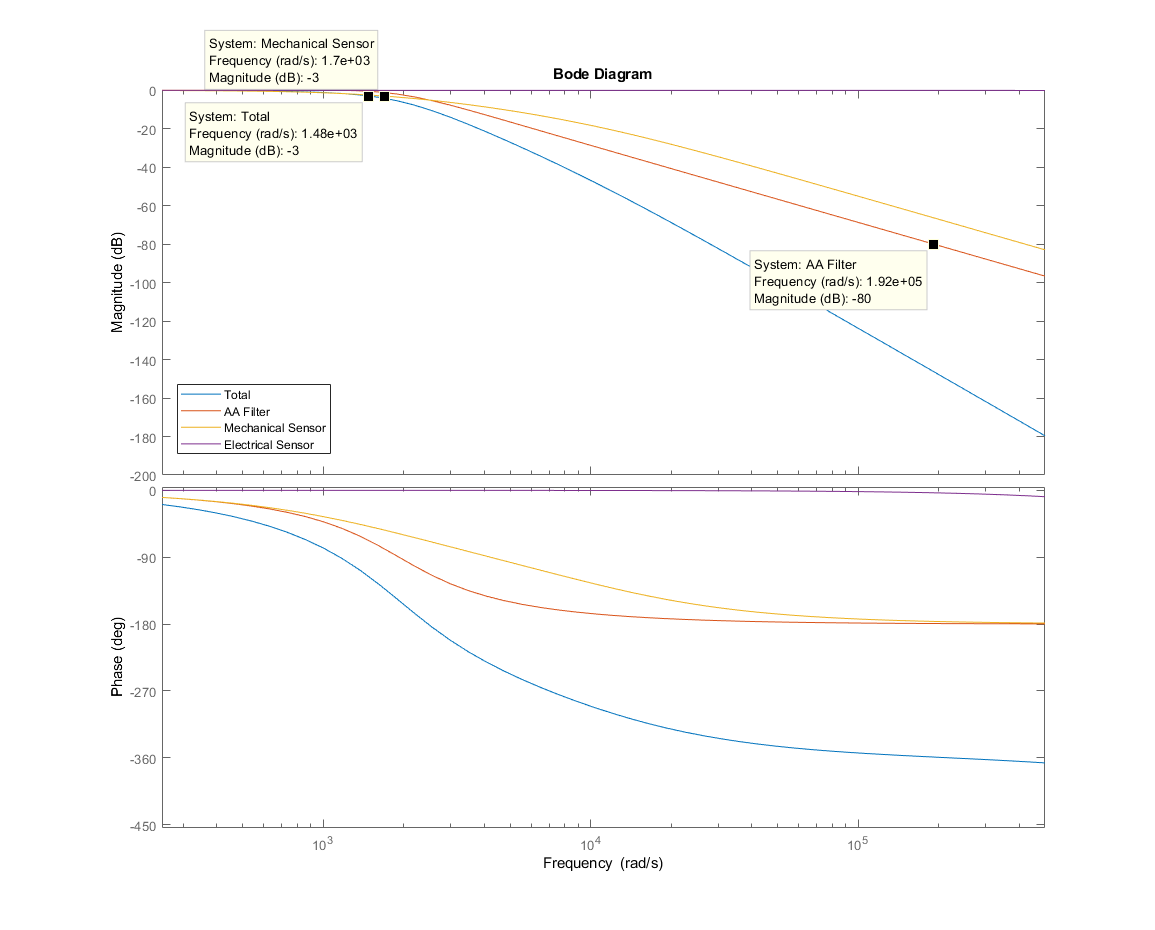
\includegraphics[width=0.5\textwidth]{bode_updated}
	\caption{Measurement system Bode plot}
	\label{fig:bode}
\end{figure}

\begin{figure}[h!]
	\centering
	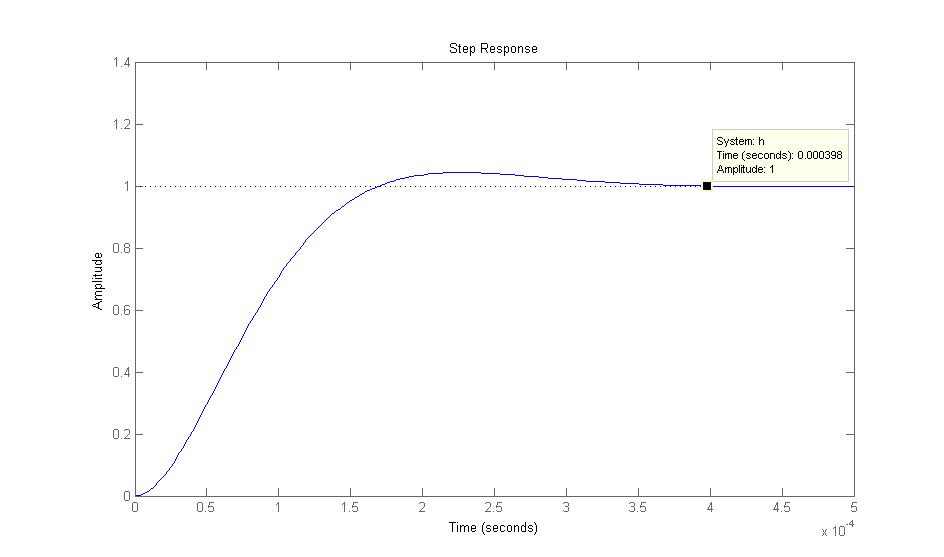
\includegraphics[width=0.5\textwidth]{filterStep}
	\caption{Measurement system step response}
	\label{fig:step}
\end{figure}

\section{Cost}

The estimated cost of the raw materials used to construct the measurement system are shown in \tabref{tab:cost}. Additional expenses incurred due to the manufacturing process and labour costs are not included in the cost breakdown.

\begin{table}[h!]
	\caption{Component costs for the measurement system} \label{tab:cost}
	\begin{tabular}{|p{0.35\textwidth}| p{0.1\textwidth}|}
		\hline
		\textbf{Component } & \textbf{Cost ($R$)} \\ \hline
		Conductive Plastic & 6.50 \\
		Wiper &  6.50 \\
		Actuator & 0.50 \\
		IN5100300 (Intai) & 189.75 \\
		$0.1\%$, 100~$\Omega$ Resistor& 92.95 \\
		$0.1\%$, 10~k$\Omega$ Resistor $\times 3$ & 78.65  \\
		$0.1\%$, 100~k$\Omega$ Resistor & 51.35\\
		$1\%$, 0.082~$\mu$F Capacitor &  29.00 \\
		$1\%$, 0.033~$\mu$F Capacitor &  23.40\\
		LMC6022 (TI) & 8.00 \\
		INA188 (TI)&  28.10 \\
		PIC24F08KM101 & 24.30 \\
		LS013B4DN04 & 140.95 \\ \hline
		\textbf{Total cost} &  \textbf{679.95} \\ \hline
	\end{tabular}
\end{table}

\section{CONCLUSION}

A potentiometric smart transducer measurement system has been designed for the purpose of measuring an electric vehicles roll angle in order to avoid a high roll-over risk. A sensor consisting of an angular potentiometer is used to convert the angular displacement measured at the wheel base into a corresponding resistance and finally an electrical current. The current is filtered using an anti-aliasing filter and sampled before being read in by an external 12-bit ADC. The information produced by the ADC is then sent to an MCU where the information is stored before being transmitted to a computer which communicates with the active safety control system already in place within the vehicle. The maximum output error of the measurement system is approximately \%. The static and dynamic characteristics of the system have been critically analysed and discussed. The total cost of the measurement system amounts to R679.95.

\bibliography{references}{}
\bibliographystyle{ieeetr}

\clearpage
\onecolumn
\appendix

\section{Circuit Diagrams}

\begin{figure}[htbp]
	\centering
	
	\def\x{6}
	\def\y{6}
	% Size of the bridge
	\def\dx{3}
	\def\dy{3}
	\begin{circuitikz}[american voltages, transform shape, scale=0.75]
		% Voltage source
		\draw (0,0) to [V, l_=$\mathrm{V_s:~51V}$]
		(0, \y) to [R, l_=$\mathrm{R_s~:~50~\Omega}$, -*] (\x, \y)
		% Left half bridge
		to [R, l_=$\mathrm{R(\theta)}$, *-] (\x-\dx,\y-\dy) % Top left resistor
		to [R, l_=$\mathrm{R_4~:~100~k\Omega}$, -*] (\x,\y-2*\dy);  % Bottom left resistor
		% Right half bridge
		\draw (\x,\y)
		to [R, l_=$\mathrm{R_2~:~100~\Omega}$] (\x+\dx, \y-\dy) % Top right resistor
		to [R, l_=$\mathrm{R_3~:~10~k\Omega}$, -*] (\x,\y-2*\dy)  % Bottom left resistor
		% Draw connection to (-) terminal of voltage source
		to (\x, 0) to (0,0);
		% Draw Vout
		\draw (\x-\dx,\y-\dy) to [short, -*] (\x-\dx+1,\y-\dy)
		(\x+3,\y-\dy) to [short, -*] (\x+2,\y-\dy);
		\draw (\x-\dx+1.5,\y-\dy) node[open] {-};
		\draw (\x+1.5,\y-\dy) node[open] {+};
		\draw (\x,\y-\dy) node[open] {$\mathrm{V_{out}}$};
		
	\end{circuitikz}
	\caption{Wheatstone bridge with resistance values}
	\label{bridge}
\end{figure}

\begin{figure} [htbp]
	\centering
	\begin{circuitikz}[transform shape,scale=.75]\draw
		(5,-0.5) node[op amp, yscale=-1](opamp){}
		(-2,0) node[left] {} to [R, l=$R_1:~10 \mathrm{k \Omega}$, o-] (0.5,0)
		to [R, l=$R_2:~10 \mathrm{k\Omega}$, -] ($(opamp.+)+(-1,0)$)
		to [C, l_=$C_2:~33~\mathrm{n F}$, -] ($(opamp.+)+(-1,-2)$) node[ground] {}	
		($(opamp.+)+(-1,0)$) to [-] (opamp.+)	
		(opamp.out) to [-] ($(opamp.out)+(0,1.5)$) 
		to [C, l_=$C_1: 82~\mathrm{n F}$, -] ($(opamp.+)+(-1,1)$)
		to [-] ($(opamp.+)+(-1,0)$)
		(opamp.-) to [-] ($(opamp.-)+(0,-1)$)
		to [-] ($(opamp.out)+(0,-1.5)$)
		to [-] (opamp.out)
		to [-o] ($(opamp.out)+(0.5,0)$)
		;	 
	\end{circuitikz}
	\caption{$2^{\mathrm{nd}}$ order AA filter.}
	\label{fig:aafilter}
\end{figure}

\begin{figure} [htbp]
	\centering
	\begin{circuitikz}[american voltages,transform shape,scale=0.75]
		\def\x{6}
		\def\y{6}
		% Size of the bridge
		\def\dx{3}
		\def\dy{3}
		\draw (19,-1.7) node[open] {LMC6022};	
		\draw
		(19,-0.5) node[op amp, yscale=-1](opamp){}
		(12,0) node[left] {} to [R, l=$10 \mathrm{k \Omega}$, -] (14,0)
		to [R, l=$10 \mathrm{k\Omega}$, -*] ($(opamp.+)+(-1,0)$)
		to [C, l_=$33~\mathrm{n F}$, -] ($(opamp.+)+(-1,-2)$) node[ground] {}	
		($(opamp.+)+(-1,0)$) to [-] (opamp.+)	
		(opamp.out) to [-] ($(opamp.out)+(0,1.5)$) 
		to [C, l_=$82~\mathrm{n F}$, -] ($(opamp.+)+(-1,1)$)
		to [-] ($(opamp.+)+(-1,0)$)
		(opamp.-) to [-] ($(opamp.-)+(0,-1)$)
		to [-] ($(opamp.out)+(0,-1.5)$)
		to [*-*] (opamp.out)
		to [*-o] ($(opamp.out)+(0.5,0)$)
		;	 
		\draw (10.5,0) node[op amp, yscale=-1](IA){}
		(12,0) to [short, -] (IA.out)
		;
		
		\draw (10.4,-1.2) node[open] {INA188};	 
		% Voltage source
		\draw (0,0) to [V, l_=$\mathrm{51V}$]
		(0, \y) to [R, l_=$\mathrm{50~\Omega}$, -*] (\x, \y)
		% Left half bridge
		to [R, l_=$\mathrm{R(\theta)}$, *-] (\x-\dx,\y-\dy) % Top left resistor
		to [R, l_=$\mathrm{100~k\Omega}$, -*] (\x,\y-2*\dy);  % Bottom left resistor
		% Right half bridge
		\draw (\x,\y)
		to [R, l_=$\mathrm{100~\Omega}$] (\x+\dx, \y-\dy) % Top right resistor
		to [R, l_=$\mathrm{10~k\Omega}$, -*] (\x,\y-2*\dy)  % Bottom left resistor
		% Draw connection to (-) terminal of voltage source
		to (\x, 0) to (0,0);
		% Draw Vout
		\draw (\x-\dx,\y-\dy) to [short, *-] (\x-\dx,-0.5) to [short, -] (IA.-)
		(\x+\dx,\y-\dy) to [short, *-] (\x+\dx,\y-2*\dy + 0.5) to [short, -] (IA.+);
		
	\end{circuitikz}
	\caption{Total circuit diagram}
	\label{fig:circuit}
\end{figure}

\end{document}